\documentclass[11pt,a4paper]{article}

% --- Packages ---
\usepackage[margin=1in]{geometry}
\usepackage{amsmath,amssymb,amsfonts}
\usepackage{booktabs}
\usepackage{graphicx}
\usepackage{hyperref}
\usepackage{xcolor}
\usepackage{caption}
\usepackage{subcaption}
\usepackage{pgfplots}
\usepackage{pgfplotstable}
\pgfplotsset{compat=1.18}
\usepgfplotslibrary{colorbrewer}

% Color definitions
\definecolor{apn-none}{HTML}{E64B35}
\definecolor{apn-tanh}{HTML}{F39B7F}
\definecolor{apn-ffn}{HTML}{B83226}
\definecolor{deltanet}{HTML}{4DBBD5}
\definecolor{deltanet-pm}{HTML}{91D1C2}
\definecolor{deltanet-ffn}{HTML}{00868B}
\definecolor{transformer}{HTML}{3C5488}
\definecolor{transformer-pm}{HTML}{8491B4}
\definecolor{gfr-k1}{HTML}{7E6148}
\definecolor{gfr-k4}{HTML}{B09C85}
\definecolor{gfr-ffn}{HTML}{DC9C6B}

\hypersetup{colorlinks=true, linkcolor=blue, citecolor=blue, urlcolor=blue}

\title{Seq-CIFAR-10 Benchmark Report:\\
Comparing APN, GFR, DeltaNet, and Transformer Architectures}
\author{Zhixin Lu}
\date{April 2026}

\begin{document}
\maketitle

% ============================================================================
\begin{abstract}
We benchmark four sequence model architectures on the sequential CIFAR-10 task:
the \textbf{Associative Plasticity Network (APN)}, a Hebbian memory model mapped onto the gated delta-rule Triton kernel;
the \textbf{Gated Forgetting Recurrence (GFR)}, a simplified element-wise gated scan model;
\textbf{DeltaNet}, a delta-rule linear attention model; and a standard \textbf{softmax Transformer} with FlashAttention-2.
All experiments use 10 layers, run for 200 epochs on a single NVIDIA H200 GPU, and share the same outer architecture.
We compare single-head and multi-head ($H{=}4$) configurations, FFN-augmented variants, and parameter-matched groups.

Key findings:
(1)~Plain APN (103K params) achieves 58.3\% test accuracy---within 5 points of the Transformer (63.5\%, 1.2M params)---while training 4$\times$ faster and using 2.7$\times$ less GPU memory.
(2)~APN is uniquely resistant to overfitting, with near-zero peak-to-final accuracy drop.
(3)~Multi-head APN ($H{=}4$) completely diverges to NaN due to unconstrained $\eta$ going negative, whereas multi-head Transformer and DeltaNet both improve (+1.7 and +0.8 points respectively).
(4)~GFR with $K{=}4$ memory slots (56.0\%) partially closes the gap with APN (58.3\%), confirming that the $D{\times}D$ matrix state provides meaningful associative capacity beyond simple exponential decay.
(5)~GFR+FFN (58.9\%) outperforms APN+FFN (56.8\%), suggesting that simpler recurrences are better suited to FFN augmentation.
(6)~Models that reach 100\% training accuracy exhibit a characteristic \emph{loss--accuracy divergence}: test loss climbs to $\sim$5.0 while test accuracy remains stable or improves, caused by increasingly confident wrong predictions on a minority of test samples.
\end{abstract}

% ============================================================================
\section{Introduction}

The Associative Plasticity Network (APN) is a biologically-inspired recurrent model that maintains a Hebbian plastic memory matrix $M_t$, updated at every time-step.
By mapping the APN recurrence onto the \emph{gated delta-rule} chunk kernel from the Flash Linear Attention (FLA) library, we achieve efficient GPU training with $O(TD)$ complexity instead of the $O(T^2 D)$ cost of standard softmax attention.

This report summarizes all 26 experiments conducted on the \textbf{Seq-CIFAR-10} benchmark, where each $32 \times 32$ CIFAR-10 image is flattened into a sequence of $T = 1024$ RGB pixels ($3$-dimensional features), and the model classifies from the last time-step.
We compare APN, GFR (a simplified scalar-memory variant), DeltaNet, and the Transformer in single-head and multi-head configurations, with and without FFN blocks, across parameter-matched groups.

% ============================================================================
\section{Model Architectures}

All models share the same outer wrapper:
\[
\texttt{Linear}(3 \to D) \;\to\; \tanh \;\to\; \underbrace{[\texttt{Layer}_i + \text{residual}]}_{i=1}^{L} \;\to\; \texttt{LayerNorm} \;\to\; \texttt{Linear}(D \to 10)
\]

\subsection{APN Layer}

The APN implements the ``$W + M$'' principle: each layer's effective weight is $W + S_t$, where $W$ is a static weight trained by backpropagation and $S_t$ is a plastic state that adapts online within the forward pass.

\paragraph{Output.}
The layer output combines static and plastic pathways:
\begin{equation}
\mathbf{o}_t = \underbrace{W^\top \text{act}(\mathbf{x}_t)}_{\mathbf{v}_t\text{ (static)}} + \underbrace{S_t^\top \text{act}(\mathbf{x}_t)}_{\text{plastic recall}} = (W + S_t)^\top \text{act}(\mathbf{x}_t)
\end{equation}

\paragraph{Plasticity rule.}
The plastic state $S_t \in \mathbb{R}^{D \times D}$ decays and updates via:
\begin{equation}\label{eq:apn-update}
S_t = \lambda \, S_{t-1} + \frac{\eta(1-\lambda)}{D} \, \mathbf{k}_t \otimes \underbrace{(\mathbf{v}_t - S_{t-1}^\top \mathbf{k}_t)}_{\mathbf{h}_t\text{ (prediction error)}}
\end{equation}
where $\mathbf{k}_t = \text{act}(\mathbf{x}_t)$, $\mathbf{v}_t = W \cdot \text{act}(\mathbf{x}_t)$, $\lambda \in (0,1)$ is a trainable decay, and $\eta$ is a trainable learning rate scalar.

\paragraph{Distinction from the original APN/APAN framework.}
The original APAN (Associative Plasticity with Attractor Networks) used a pure Hebbian update where the learning signal was the layer's full output: $\mathbf{h}_t = \mathbf{v}_t + S_{t-1}^\top \mathbf{k}_t$.
The implemented APN instead uses the \emph{prediction error} $\mathbf{h}_t = \mathbf{v}_t - S_{t-1}^\top \mathbf{k}_t$ as the learning signal---the difference between what the static weight predicts and what the plastic memory already recalls.

The reason for this change is \textbf{stability}: the original Hebbian form creates positive feedback (the recall amplifies itself through the update), making the system conditionally unstable when $\|\mathbf{k}\|^2 \geq d/\eta$.
The prediction-error form provides negative feedback: once the plastic memory has learned an association ($S^\top \mathbf{k} \approx \mathbf{v}$), the update vanishes automatically.
This makes the recurrence unconditionally stable for $\eta > 0$.

The rule remains Hebbian in the broad sense---it is a rank-one outer product of pre-synaptic activity ($\mathbf{k}$) and a post-synaptic signal ($\mathbf{h}$)---but the post-synaptic signal is a \emph{surprise/novelty} signal rather than the raw output.
The ``$W + M$'' interpretation is preserved: $W$ encodes innate/trained knowledge, $S$ accumulates experience within a sequence, and the effective weight $(W + S_t)$ grows richer over time.

\textbf{Parameters per layer:} $D^2$ (one linear projection $W$) $+ 2D$ (LayerNorm) $+ 2$ (scalars $\eta, \lambda$) $\approx D^2$.

\subsection{GFR Layer (Gated Forgetting Recurrence)}

Each GFR layer maintains $K$ scalar memory slots per neuron (total state: $D \cdot K$ scalars):
\begin{equation}
m_{i,k,t} = \lambda_k \, m_{i,k,t-1} + z_{i,t}, \quad
h_{i,t} = z_{i,t} + \sum_{k=1}^{K} \eta_k \, m_{i,k,t}
\end{equation}
where $\mathbf{z}_t = W \cdot \text{act}(\mathbf{x}_t)$ is the projected input. This uses the HGRN chunk kernel (simple element-wise gated prefix scan).

\textbf{Parameters per layer:} $D^2$ (projection $W$) $+ 2K$ (scalars $\lambda, \eta$) $+ 2D$ (LayerNorm) $\approx D^2$.

\subsection{DeltaNet Layer}

DeltaNet uses separate Q/K/V projections with the (non-gated) delta rule:
\begin{equation}
S_t = S_{t-1} + \beta_t \, \mathbf{k}_t \otimes \bigl(\mathbf{v}_t - S_{t-1}^\top \mathbf{k}_t\bigr), \quad \mathbf{o}_t = \mathbf{q}_t^\top S_t
\end{equation}
where $\beta_t = \sigma(W_\beta \mathbf{x}_t)$ is a learned, input-dependent step size.

\textbf{Parameters per layer:} $3D^2$ (Q/K/V projections) $+ D$ ($\beta$ projection) $+ 2D$ (LayerNorm) $\approx 3D^2$.

\subsection{Transformer Layer}

A pre-norm causal Transformer block with FlashAttention-2:
\[
\texttt{LN} \to \texttt{MHA} \to \text{residual} \to \texttt{LN} \to \texttt{FFN}(D \to 4D \to D) \to \text{residual}
\]

\textbf{Parameters per layer:} $4D^2$ (QKV + output proj) $+ 8D^2$ (FFN) $+ 4D$ (two LayerNorms) $\approx 12D^2$.

\subsection{Parameter Count Summary}

\begin{table}[h]
\centering
\caption{Parameters per layer and total model parameters ($L=10$).}
\label{tab:params}
\begin{tabular}{lccc}
\toprule
\textbf{Model} & \textbf{Per-layer} & \textbf{Total (10L)} & \textbf{Relative} \\
\midrule
\multicolumn{4}{l}{\textit{No FFN ($\approx$103K parameter-matched)}} \\
\midrule
APN ($D=100$) & $\approx D^2 = 10$K & 103,630 & $1\times$ \\
GFR $K{=}1$ ($D=100$) & $\approx D^2 = 10$K & 103,630 & $1\times$ \\
GFR $K{=}4$ per-slot ($D=100$) & $\approx D^2 = 10$K & 103,690 & $1\times$ \\
DeltaNet ($D=58$) & $\approx 3D^2 = 10$K & 103,598 & $1\times$ \\
Transformer ($D=29$) & $\approx 12D^2 = 10$K & 102,554 & $1\times$ \\
\midrule
\multicolumn{4}{l}{\textit{With FFN ($\approx$1.2M parameter-matched)}} \\
\midrule
APN + FFN ($D=115$) & $\approx 9D^2$ & 1,196,720 & $11.5\times$ \\
GFR $K{=}1$ + FFN ($D=115$) & $\approx 9D^2$ & 1,196,720 & $11.5\times$ \\
DeltaNet + FFN ($D=104$) & $\approx 11D^2$ & 1,196,634 & $11.5\times$ \\
Transformer ($D=100$) & $\approx 12D^2$ & 1,205,610 & $11.6\times$ \\
\midrule
\multicolumn{4}{l}{\textit{Width-matched ($D=100$, no FFN)}} \\
\midrule
DeltaNet ($D=100$) & $\approx 3D^2 = 30$K & 304,610 & $2.9\times$ \\
\bottomrule
\end{tabular}
\end{table}

% ============================================================================
\section{Experimental Setup}

\begin{itemize}
\item \textbf{Hardware:} Single NVIDIA H200 GPU (141 GB HBM3e, 228 KB shared memory per SM)
\item \textbf{Task:} Seq-CIFAR-10 (1024-step sequences, 10-class classification)
\item \textbf{Optimizer:} AdamW ($\text{lr} = 10^{-3}$, weight decay $= 10^{-4}$, grad clip $= 1.0$)
\item \textbf{Schedule:} Cosine annealing with 20-epoch linear warmup (unless noted)
\item \textbf{Batch size:} 64
\item \textbf{Epochs:} 200
\item \textbf{Seed:} 42
\item \textbf{Triton version:} $\ge$3.3.0, $<$3.4.0 (pinned due to Hopper backward kernel bug in $\ge$3.4)
\end{itemize}

% ============================================================================
\section{Results}

\subsection{Complete Results Summary}

\begin{table}[h]
\centering
\caption{All 26 experiments (200 epochs unless noted). Bold: best per group. ``Drop'' = peak $-$ final test accuracy.}
\label{tab:results}
\resizebox{\textwidth}{!}{%
\begin{tabular}{llcccccccc}
\toprule
\textbf{Model} & \textbf{Config} & \textbf{$D$} & \textbf{$H$} & \textbf{Params} & \textbf{Peak Acc (\%)} & \textbf{Peak Ep} & \textbf{Final Acc (\%)} & \textbf{Drop} & \textbf{s/ep} \\
\midrule
\multicolumn{10}{l}{\textit{Group 1: $\approx$1.2M params (with FFN or large Transformer)}} \\
\midrule
Transformer & $H{=}4$, warmup20 & 100 & 4 & 1,205,610 & \textbf{65.16} & 183 & 65.13 & 0.03 & 85.1 \\
Transformer & $H{=}1$, warmup20 & 100 & 1 & 1,205,610 & 63.50 & 180 & 63.46 & 0.04 & 39.3 \\
DeltaNet+FFN & $H{=}4$, warmup20 & 104 & 4 & 1,199,754 & 63.56 & 145 & 63.39 & 0.17 & 59.1 \\
DeltaNet+FFN & $H{=}1$, warmup20 & 104 & 1 & 1,196,634 & 62.80 & 198 & 62.80 & 0.00 & 112.1 \\
GFR $K{=}1$+FFN & warmup20 & 115 & 1 & 1,196,720 & 58.93 & 192 & 58.75 & 0.18 & 33.3 \\
APN+FFN & $H{=}1$, warmup20 & 115 & 1 & 1,196,720 & 56.84 & 177 & 56.68 & 0.16 & 55.3 \\
APN+FFN & $H{=}4$, per-head & 116 & 4 & 1,217,626 & 40.58$^\dagger$ & 9 & 10.00 & --- & 37.7 \\
\midrule
\multicolumn{10}{l}{\textit{Group 2: $\approx$103K params (no FFN, parameter-matched)}} \\
\midrule
DeltaNet & param-match & 58 & 1 & 103,598 & 60.06 & 18 & 55.40 & 4.66 & 69.0 \\
Transformer & param-match, warmup20 & 29 & 1 & 102,554 & 59.75 & 38 & 55.89 & 3.86 & 32.6 \\
APN & \textbf{act=none, warmup20} & 100 & 1 & 103,630 & \textbf{58.34} & 189 & 58.17 & 0.17 & 25.5 \\
APN & act=none, no warmup & 100 & 1 & 103,630 & 58.12 & 163 & 57.96 & 0.16 & 26.0 \\
GFR $K{=}1$+FFN & $D{=}34$, warmup20 & 34 & 1 & 105,974 & 57.57 & 39 & 51.89 & 5.68 & 18.9 \\
GFR $K{=}4$ & per-slot, warmup20 & 100 & 1 & 103,690 & 56.00 & 199 & 55.70 & 0.30 & 22.7 \\
GFR $K{=}4$ & per-neuron, warmup20 & 100 & 1 & 111,610 & 56.21 & 196 & 55.56 & 0.65 & 22.8 \\
GFR $K{=}1$ & per-slot, warmup20 & 100 & 1 & 103,630 & 53.57 & 199 & 53.01 & 0.56 & 14.0 \\
GFR $K{=}1$ & per-neuron, warmup20 & 100 & 1 & 105,610 & 52.43 & 189 & 51.73 & 0.70 & 14.0 \\
APN & act=tanh, better init & 100 & 1 & 103,630 & 53.15 & 168 & 52.50 & 0.65 & 80.1 \\
APN & act=tanh & 100 & 1 & 103,630 & 51.69 & 162 & 51.16 & 0.53 & 26.2 \\
APN & $H{=}4$, per-head & 100 & 4 & 103,690 & 10.00$^\dagger$ & --- & 10.00 & --- & 26.1 \\
\midrule
\multicolumn{10}{l}{\textit{Group 3: Width-matched ($D{=}100$, no FFN)}} \\
\midrule
DeltaNet & no warmup & 100 & 1 & 304,610 & 62.28 & 11 & 60.80 & 1.48 & 100.4 \\
DeltaNet & warmup20 & 100 & 1 & 304,610 & 59.26 & 21 & 58.73 & 0.53 & 100.4 \\
APN & act=none, warmup20 & 100 & 1 & 103,630 & 58.34 & 189 & 58.17 & 0.17 & 25.5 \\
\bottomrule
\end{tabular}%
}

\smallskip
{\footnotesize ${}^\dagger$ Diverged to NaN during training (see Section~\ref{sec:nan}).}
\end{table}

% ============================================================================
\subsection{Key Finding 1: APN Is the Most Parameter-Efficient Model}

\begin{figure}[h]
\centering
\begin{tikzpicture}
\begin{axis}[
    width=0.85\textwidth,
    height=0.55\textwidth,
    xlabel={Epoch},
    ylabel={Test Accuracy (\%)},
    xmin=0, xmax=200,
    ymin=35, ymax=62,
    grid=major,
    grid style={gray!30},
    legend style={at={(0.98,0.02)}, anchor=south east, font=\footnotesize, draw=none, fill=white, fill opacity=0.8},
    every axis plot/.append style={thick},
    title={\textbf{Parameter-matched group ($\approx$103K params, no FFN)}},
    title style={font=\normalsize},
]

\addplot[color=apn-none, thick] table[x=epoch, y=test/acc, col sep=comma]
    {../report_data/apn_L10_D100_H200_B64_act-none_warmup20.csv};
\addlegendentry{APN act=none (103K)}

\addplot[color=deltanet-pm, thick] table[x=epoch, y=test/acc, col sep=comma]
    {../report_data/deltanet_L10_D58_H200_B64.csv};
\addlegendentry{DeltaNet D=58 (104K)}

\addplot[color=transformer-pm, thick] table[x=epoch, y=test/acc, col sep=comma]
    {../report_data/transformer_L10_D29_H200_B64_warmup20_paramatch.csv};
\addlegendentry{Transformer D=29 (103K)}

\addplot[color=gfr-k4, thick] table[x=epoch, y=test/acc, col sep=comma]
    {../report_data/gfr_K4_D100_perslot.csv};
\addlegendentry{GFR K=4 per-slot (104K)}

\addplot[color=gfr-k1, thick, dashed] table[x=epoch, y=test/acc, col sep=comma]
    {../report_data/gfr_K1_D100.csv};
\addlegendentry{GFR K=1 (104K)}

\end{axis}
\end{tikzpicture}
\caption{Test accuracy for parameter-matched models ($\approx$103K). APN (act=none) converges steadily to 58.3\%, while DeltaNet peaks early (epoch 18) and declines 4.7 points by epoch 200. The Transformer also peaks early (epoch 38) and declines 3.9 points. APN and GFR models show minimal overfitting.}
\label{fig:paramatch}
\end{figure}

With only 103K parameters, APN (act=none) achieves 58.34\% test accuracy.
DeltaNet requires $3\times$ the parameters (305K) to reach 62.28\%, and the Transformer requires $12\times$ (1.2M) to reach 63.50\%.
Per 1K parameters, APN extracts 0.56\% accuracy, versus 0.20\% for DeltaNet and 0.053\% for the Transformer.
Moreover, APN's peak occurs at epoch 189 with only a 0.17-point drop by epoch 200---it requires no early stopping.
In contrast, DeltaNet $D{=}58$ drops 4.66 points and the Transformer $D{=}29$ drops 3.86 points from their peaks.

% ============================================================================
\subsection{Key Finding 2: FFN Helps DeltaNet and GFR but Hurts APN}

\begin{figure}[h]
\centering
\begin{tikzpicture}
\begin{axis}[
    width=0.85\textwidth,
    height=0.55\textwidth,
    xlabel={Epoch},
    ylabel={Test Accuracy (\%)},
    xmin=0, xmax=200,
    ymin=35, ymax=67,
    grid=major,
    grid style={gray!30},
    legend style={at={(0.98,0.02)}, anchor=south east, font=\footnotesize, draw=none, fill=white, fill opacity=0.8},
    every axis plot/.append style={thick},
    title={\textbf{FFN-augmented group ($\approx$1.2M params)}},
    title style={font=\normalsize},
]

\addplot[color=transformer, thick] table[x=epoch, y=test/acc, col sep=comma]
    {../report_data/transformer_L10_D100_H200_B64_warmup20.csv};
\addlegendentry{Transformer D=100 (1.2M)}

\addplot[color=deltanet-ffn, thick] table[x=epoch, y=test/acc, col sep=comma]
    {../report_data/deltanet_L10_D104_H200_B64_ffn_warmup20_paramatch.csv};
\addlegendentry{DeltaNet+FFN D=104 (1.2M)}

\addplot[color=gfr-ffn, thick] table[x=epoch, y=test/acc, col sep=comma]
    {../report_data/gfr_K1_D115_ffn.csv};
\addlegendentry{GFR K=1+FFN D=115 (1.2M)}

\addplot[color=apn-ffn, thick] table[x=epoch, y=test/acc, col sep=comma]
    {../report_data/apn_L10_D115_H200_B64_ffn_warmup20_paramatch.csv};
\addlegendentry{APN+FFN D=115 (1.2M)}

\addplot[color=apn-none, thick, dashed] table[x=epoch, y=test/acc, col sep=comma]
    {../report_data/apn_L10_D100_H200_B64_act-none_warmup20.csv};
\addlegendentry{APN no-FFN D=100 (103K, reference)}

\end{axis}
\end{tikzpicture}
\caption{FFN-augmented models at $\approx$1.2M params. DeltaNet+FFN (62.8\%) nearly matches the Transformer (63.5\%). GFR+FFN (58.9\%) benefits from the FFN. Remarkably, APN+FFN (56.8\%, solid dark red) \emph{underperforms} plain APN without FFN (58.3\%, dashed red) despite having 12$\times$ more parameters.}
\label{fig:ffn}
\end{figure}

At $\approx$1.2M parameters, all FFN-augmented models reach 100\% training accuracy.
The critical difference is generalization:
\begin{itemize}
\item \textbf{DeltaNet+FFN (62.80\%)} nearly matches the Transformer (63.50\%), only 0.7 points behind.
\item \textbf{GFR+FFN (58.93\%)} benefits from the FFN, outperforming plain GFR $K{=}1$ by 5.4 points---and outperforming APN+FFN by 2.1 points.
\item \textbf{APN+FFN (56.84\%)} is \emph{worse} than plain APN (58.34\%) by 1.5 points despite 12$\times$ more parameters.
\end{itemize}
The FFN enables 100\% train accuracy for APN, but this capacity is entirely wasted on memorization.
APN's single-projection tied key-value design ($\mathbf{k} = \mathbf{v} = W\mathbf{x}$) produces representations too constrained for the FFN to refine productively.
In contrast, GFR's simpler element-wise recurrence produces features that the FFN can meaningfully transform.

% ============================================================================
\subsection{Key Finding 3: Multi-Head Improves Transformer and DeltaNet but Destabilizes APN}
\label{sec:nan}

\begin{figure}[h]
\centering
\begin{tikzpicture}
\begin{axis}[
    width=0.85\textwidth,
    height=0.55\textwidth,
    xlabel={Epoch},
    ylabel={Test Accuracy (\%)},
    xmin=0, xmax=200,
    ymin=35, ymax=67,
    grid=major,
    grid style={gray!30},
    legend style={at={(0.02,0.98)}, anchor=north west, font=\footnotesize, draw=none, fill=white, fill opacity=0.8},
    every axis plot/.append style={thick},
    title={\textbf{Multi-head ($H{=}4$) vs.\ single-head ($H{=}1$)}},
    title style={font=\normalsize},
]

\addplot[color=transformer, thick] table[x=epoch, y=test/acc, col sep=comma]
    {../report_data/transformer_D100_H4.csv};
\addlegendentry{Transformer H=4 (65.2\%)}

\addplot[color=transformer-pm, thick, dashed] table[x=epoch, y=test/acc, col sep=comma]
    {../report_data/transformer_L10_D100_H200_B64_warmup20.csv};
\addlegendentry{Transformer H=1 (63.5\%)}

\addplot[color=deltanet-ffn, thick] table[x=epoch, y=test/acc, col sep=comma]
    {../report_data/deltanet_D104_H4_ffn.csv};
\addlegendentry{DeltaNet+FFN H=4 (63.6\%)}

\addplot[color=deltanet-pm, thick, dashed] table[x=epoch, y=test/acc, col sep=comma]
    {../report_data/deltanet_L10_D104_H200_B64_ffn_warmup20_paramatch.csv};
\addlegendentry{DeltaNet+FFN H=1 (62.8\%)}

\end{axis}
\end{tikzpicture}
\caption{Multi-head ($H{=}4$) vs.\ single-head. Transformer improves from 63.5\% to 65.2\% (+1.7 points). DeltaNet+FFN improves from 62.8\% to 63.6\% (+0.8 points). APN $H{=}4$ diverges to NaN and is not shown (see text).}
\label{fig:multihead}
\end{figure}

Multi-head attention ($H{=}4$) benefits the Transformer (+1.66 points, from 63.50\% to 65.16\%) and DeltaNet+FFN (+0.76 points, from 62.80\% to 63.56\%).
However, \textbf{both multi-head APN runs diverged completely}:

\begin{itemize}
\item \textbf{APN $H{=}4$ without FFN} ($D{=}100$): NaN from epoch 1. All scalars immediately become NaN.
\item \textbf{APN $H{=}4$ with FFN} ($D{=}116$): Trains for 9 epochs (peak 40.6\% at epoch 9), then NaN at epoch 10. The scalar logs reveal that head~3's $\eta$ (initialized at 0.1) \emph{goes negative} ($-0.12$ at epoch 9), causing the Hebbian update to amplify rather than correct errors. Meanwhile, head~0's $\eta$ (initialized at 1.0 with $\lambda{=}0.999$) grows unboundedly ($1.08$ at epoch 9).
\end{itemize}

\textbf{Root cause analysis.} With $H{=}4$, each head operates on a $D/H = 25$-dimensional subspace with a $25 \times 25$ state matrix.
The Hebbian outer-product update $\mathbf{k}_t \otimes (\mathbf{v}_t - S_{t-1}^\top \mathbf{k}_t)$ amplifies noise when:
(1)~the per-head dimension is too small, making the rank-1 update dominate the state;
(2)~$\eta$ is unconstrained and can go negative, reversing the sign of the delta correction;
(3)~$\lambda{=}0.9$ (head~2's initialization) provides insufficient damping, so errors accumulate rapidly.
For the no-FFN variant, the $25{\times}25$ state is so small that the system is unstable from the first gradient step.
These issues do not affect DeltaNet because its $\beta_t = \sigma(\cdot) \in (0,1)$ is always positive and bounded.

% ============================================================================
\subsection{Key Finding 4: GFR Validates the Importance of APN's Matrix State}

\begin{figure}[h]
\centering
\begin{tikzpicture}
\begin{axis}[
    width=0.85\textwidth,
    height=0.55\textwidth,
    xlabel={Epoch},
    ylabel={Test Accuracy (\%)},
    xmin=0, xmax=200,
    ymin=35, ymax=60,
    grid=major,
    grid style={gray!30},
    legend style={at={(0.98,0.02)}, anchor=south east, font=\footnotesize, draw=none, fill=white, fill opacity=0.8},
    every axis plot/.append style={thick},
    title={\textbf{APN vs.\ GFR variants ($\approx$103K params, no FFN)}},
    title style={font=\normalsize},
]

\addplot[color=apn-none, thick] table[x=epoch, y=test/acc, col sep=comma]
    {../report_data/apn_L10_D100_H200_B64_act-none_warmup20.csv};
\addlegendentry{APN act=none (58.3\%)}

\addplot[color=gfr-k4, thick] table[x=epoch, y=test/acc, col sep=comma]
    {../report_data/gfr_K4_D100_perslot.csv};
\addlegendentry{GFR K=4 per-slot (56.0\%)}

\addplot[color=gfr-k4, thick, dashed] table[x=epoch, y=test/acc, col sep=comma]
    {../report_data/gfr_K4_D100_perneuron.csv};
\addlegendentry{GFR K=4 per-neuron (56.2\%)}

\addplot[color=gfr-k1, thick] table[x=epoch, y=test/acc, col sep=comma]
    {../report_data/gfr_K1_D100.csv};
\addlegendentry{GFR K=1 per-slot (53.6\%)}

\addplot[color=gfr-k1, thick, dashed] table[x=epoch, y=test/acc, col sep=comma]
    {../report_data/gfr_K1_D100_perneuron.csv};
\addlegendentry{GFR K=1 per-neuron (52.4\%)}

\end{axis}
\end{tikzpicture}
\caption{APN vs.\ GFR variants at matched parameters. APN's $D{\times}D$ matrix state outperforms GFR's scalar memory slots by 2.3--5.9 points. Adding slots ($K{=}4$) helps significantly (+2.4 points over $K{=}1$), partially compensating for the lack of associative capacity. Per-neuron parameterization offers no clear advantage over per-slot.}
\label{fig:gfr}
\end{figure}

GFR serves as an ablation of APN, replacing the $D \times D$ matrix state with $K$ independent exponentially-decaying scalar memories.
The results confirm that \textbf{APN's matrix state provides meaningful associative capacity}:
\begin{itemize}
\item GFR $K{=}1$: 53.57\% ($-4.8$ points vs.\ APN). A single exponential decay cannot perform the delta-rule error correction.
\item GFR $K{=}4$ per-slot: 56.00\% ($-2.3$ points). Multiple timescales partially compensate by allowing the model to store short- and long-term features simultaneously.
\item GFR $K{=}4$ per-neuron: 56.21\% ($-2.1$ points). Per-neuron parameters (800 extra per layer) do not meaningfully outperform the simpler per-slot parameterization (8 extra per layer).
\item GFR $K{=}1$ per-neuron: 52.43\% ($-5.9$ points). Worse than per-slot $K{=}1$, suggesting that per-neuron decay rates with a single slot overfit.
\end{itemize}

GFR is significantly faster than APN: 14.0 s/epoch for $K{=}1$ (vs.\ 25.5 s for APN) and 22.7 s for $K{=}4$.
The HGRN kernel's element-wise scan is computationally trivial compared to APN's tiled $D \times D$ delta-rule computation.

% ============================================================================
\subsection{Key Finding 5: Loss--Accuracy Divergence in Overparameterized Models}
\label{sec:loss_divergence}

\begin{figure}[h]
\centering
\begin{subfigure}[b]{0.48\textwidth}
\begin{tikzpicture}
\begin{axis}[
    width=\textwidth,
    height=0.75\textwidth,
    xlabel={Epoch},
    ylabel={Test Accuracy (\%)},
    xmin=0, xmax=200,
    ymin=35, ymax=67,
    grid=major,
    grid style={gray!30},
    legend style={at={(0.98,0.02)}, anchor=south east, font=\tiny, draw=none, fill=white, fill opacity=0.8},
    every axis plot/.append style={thick},
]
\addplot[color=transformer, thick] table[x=epoch, y=test/acc, col sep=comma]
    {../report_data/transformer_D100_H4.csv};
\addlegendentry{Transformer H=4}
\addplot[color=deltanet-ffn, thick] table[x=epoch, y=test/acc, col sep=comma]
    {../report_data/deltanet_D104_H4_ffn.csv};
\addlegendentry{DeltaNet+FFN H=4}
\addplot[color=gfr-ffn, thick] table[x=epoch, y=test/acc, col sep=comma]
    {../report_data/gfr_K1_D115_ffn.csv};
\addlegendentry{GFR+FFN}
\end{axis}
\end{tikzpicture}
\caption{Test accuracy continues improving}
\end{subfigure}
\hfill
\begin{subfigure}[b]{0.48\textwidth}
\begin{tikzpicture}
\begin{axis}[
    width=\textwidth,
    height=0.75\textwidth,
    xlabel={Epoch},
    ylabel={Test Loss (CE)},
    xmin=0, xmax=200,
    ymin=0.5, ymax=6.0,
    grid=major,
    grid style={gray!30},
    legend style={at={(0.02,0.98)}, anchor=north west, font=\tiny, draw=none, fill=white, fill opacity=0.8},
    every axis plot/.append style={thick},
]
\addplot[color=transformer, thick] table[x=epoch, y=test/loss, col sep=comma]
    {../report_data/transformer_D100_H4.csv};
\addlegendentry{Transformer H=4}
\addplot[color=deltanet-ffn, thick] table[x=epoch, y=test/loss, col sep=comma]
    {../report_data/deltanet_D104_H4_ffn.csv};
\addlegendentry{DeltaNet+FFN H=4}
\addplot[color=gfr-ffn, thick] table[x=epoch, y=test/loss, col sep=comma]
    {../report_data/gfr_K1_D115_ffn.csv};
\addlegendentry{GFR+FFN}
\end{axis}
\end{tikzpicture}
\caption{Test loss diverges to $\sim$5.0--5.5}
\end{subfigure}
\caption{Loss--accuracy divergence in overparameterized models. All three models reach 100\% train accuracy and develop increasingly confident predictions. On test samples where the model is wrong, the large logit magnitudes produce enormous cross-entropy loss. Since accuracy only measures correct/incorrect (not confidence), test accuracy can improve even as test loss explodes. Final test losses: Transformer H=4: 5.49, DeltaNet+FFN H=4: 5.19, GFR+FFN: 5.31.}
\label{fig:loss_divergence}
\end{figure}

A striking phenomenon in our experiments: models that achieve 100\% training accuracy show test loss climbing to $\sim$5.0--5.5 in later epochs, while test accuracy remains stable or even improves slightly.
This occurs in the Transformer ($H{=}4$: final test loss 5.49, acc 65.1\%), DeltaNet+FFN ($H{=}4$: loss 5.19, acc 63.4\%), and GFR+FFN (loss 5.31, acc 58.8\%).

\textbf{Explanation.} Cross-entropy loss is $-\log p_{\text{correct}}$.
When a model reaches 100\% train accuracy with near-zero train loss ($\sim 10^{-9}$), its logits become very large in magnitude.
On test samples, the model is still correct on $\sim$63--65\% of examples (producing near-zero per-sample loss for those), but for the $\sim$35\% of misclassified samples, the large logit magnitudes mean the model is \emph{confidently wrong}, yielding per-sample losses of $\sim$15--20.
The mean across all samples produces the observed $\sim$5.0 test loss.
Accuracy only counts the argmax and is insensitive to confidence, so it remains stable.

\textbf{Notably, APN and GFR without FFN never exhibit this divergence} (final test losses $\sim$1.2--1.3) because they cannot reach 100\% train accuracy---their implicit regularization prevents the logit magnitudes from growing unboundedly.

% ============================================================================
\subsection{Speed and Memory Comparison}

\begin{figure}[h]
\centering
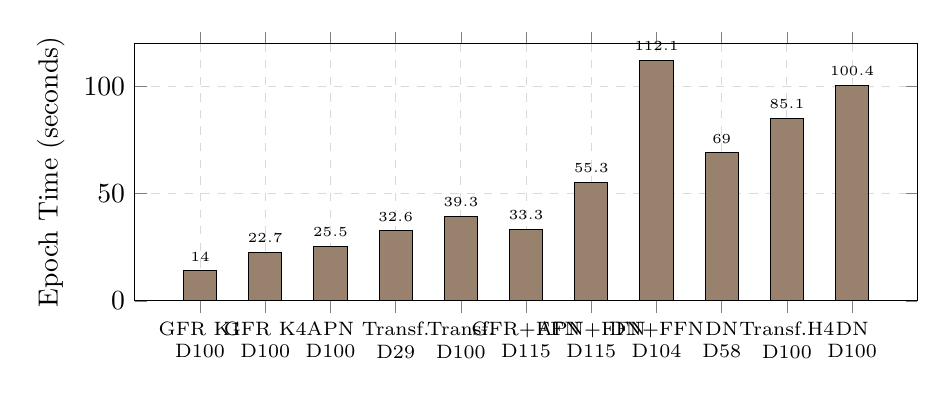
\begin{tikzpicture}
\begin{axis}[
    ybar,
    width=0.95\textwidth,
    height=0.4\textwidth,
    ylabel={Epoch Time (seconds)},
    symbolic x coords={GFR K1\\D100, GFR K4\\D100, APN\\D100, Transf.\\D29, Transf.\\D100, GFR+FFN\\D115, APN+FFN\\D115, DN+FFN\\D104, DN\\D58, Transf.H4\\D100, DN\\D100},
    xtick=data,
    x tick label style={align=center, font=\scriptsize},
    ymin=0, ymax=120,
    bar width=12pt,
    nodes near coords,
    nodes near coords style={font=\tiny, above},
    grid=major,
    grid style={gray!30, dashed},
]
\addplot[fill=gfr-k1!80] coordinates {
    (GFR K1\\D100, 14.0)
    (GFR K4\\D100, 22.7)
    (APN\\D100, 25.5)
    (Transf.\\D29, 32.6)
    (Transf.\\D100, 39.3)
    (GFR+FFN\\D115, 33.3)
    (APN+FFN\\D115, 55.3)
    (DN+FFN\\D104, 112.1)
    (DN\\D58, 69.0)
    (Transf.H4\\D100, 85.1)
    (DN\\D100, 100.4)
};
\end{axis}
\end{tikzpicture}
\caption{Training time per epoch (lower is better). GFR $K{=}1$ is the fastest (14s), followed by GFR $K{=}4$ (23s) and APN (26s). DeltaNet is consistently the slowest due to its Triton kernel overhead at these dimensions.}
\label{fig:epoch_time}
\end{figure}

\begin{table}[h]
\centering
\caption{Speed and memory comparison for key configurations.}
\label{tab:speed_memory}
\begin{tabular}{lccc}
\toprule
\textbf{Model (params)} & \textbf{s/epoch} & \textbf{Peak GPU (MB)} & \textbf{Relative speed} \\
\midrule
GFR $K{=}1$ $D{=}100$ (104K) & 14.0 & 1,460 & 1.0$\times$ (fastest) \\
GFR $K{=}4$ $D{=}100$ (104K) & 22.7 & 3,154 & 1.6$\times$ \\
APN $D{=}100$ (104K) & 25.5 & 1,590 & 1.8$\times$ \\
Transformer $D{=}29$ (103K) & 32.6 & 4,623 & 2.3$\times$ \\
Transformer $D{=}100$ (1.2M) & 39.3 & 4,278 & 2.8$\times$ \\
DeltaNet $D{=}58$ (104K) & 69.0 & 1,151 & 4.9$\times$ \\
DeltaNet $D{=}100$ (305K) & 100.4 & 2,133 & 7.2$\times$ \\
Transformer $H{=}4$ $D{=}100$ (1.2M) & 85.1 & 17,158 & 6.1$\times$ \\
\bottomrule
\end{tabular}
\end{table}

Key observations:
\begin{itemize}
\item \textbf{GFR $K{=}1$ is fastest} at 14s/epoch---$1.8\times$ faster than APN and $7\times$ faster than DeltaNet.
\item \textbf{APN is 4$\times$ faster than DeltaNet} at the same width ($D{=}100$), due to its single projection vs.\ three.
\item \textbf{Transformer $H{=}4$ uses 17 GB} GPU memory---$4\times$ more than $H{=}1$ (4.3 GB)---because FlashAttention-2's $H{=}4$ configuration stores more intermediate activations for the backward pass.
\item \textbf{GFR $K{=}4$ uses 3.2 GB}---$2\times$ more than $K{=}1$ (1.5 GB)---proportional to the $4\times$ larger state vector.
\end{itemize}

% ============================================================================
\subsection{APN Scalar Dynamics}

\begin{figure}[h]
\centering
\begin{subfigure}[b]{0.48\textwidth}
\begin{tikzpicture}
\begin{axis}[
    width=\textwidth,
    height=0.7\textwidth,
    xlabel={Epoch},
    ylabel={$\eta$},
    xmin=0, xmax=200,
    grid=major,
    grid style={gray!30},
    legend style={at={(0.02,0.98)}, anchor=north west, font=\footnotesize, draw=none, fill=white, fill opacity=0.8},
    every axis plot/.append style={thick},
]
\addplot[color=apn-none, thick] table[x=epoch, y=apn/eta_layer0, col sep=comma]
    {../report_data/apn_L10_D100_H200_B64_act-none_warmup20_scalars.csv};
\addlegendentry{Layer 0}
\addplot[color=transformer, thick, dashed] table[x=epoch, y=apn/eta_layer9, col sep=comma]
    {../report_data/apn_L10_D100_H200_B64_act-none_warmup20_scalars.csv};
\addlegendentry{Layer 9}
\end{axis}
\end{tikzpicture}
\caption{Learned $\eta$ (APN act=none)}
\end{subfigure}
\hfill
\begin{subfigure}[b]{0.48\textwidth}
\begin{tikzpicture}
\begin{axis}[
    width=\textwidth,
    height=0.7\textwidth,
    xlabel={Epoch},
    ylabel={$\lambda$},
    xmin=0, xmax=200,
    ymin=0.990, ymax=1.001,
    grid=major,
    grid style={gray!30},
    legend style={at={(0.02,0.02)}, anchor=south west, font=\footnotesize, draw=none, fill=white, fill opacity=0.8},
    every axis plot/.append style={thick},
]
\addplot[color=apn-none, thick] table[x=epoch, y=apn/lam_layer0, col sep=comma]
    {../report_data/apn_L10_D100_H200_B64_act-none_warmup20_scalars.csv};
\addlegendentry{Layer 0}
\addplot[color=transformer, thick, dashed] table[x=epoch, y=apn/lam_layer9, col sep=comma]
    {../report_data/apn_L10_D100_H200_B64_act-none_warmup20_scalars.csv};
\addlegendentry{Layer 9}
\end{axis}
\end{tikzpicture}
\caption{Learned $\lambda$ (APN act=none)}
\end{subfigure}
\caption{Evolution of APN scalars during training. Both $\eta$ and $\lambda$ remain close to their initializations ($\eta{=}1.0$, $\lambda{=}0.999$), confirming the initialization is near-optimal. $\lambda$ converges toward 1.0 (minimal forgetting), consistent with the Seq-CIFAR-10 task requiring information from the entire 1024-step sequence.}
\label{fig:scalars}
\end{figure}

% ============================================================================
\section{Activation Function Analysis}

\begin{table}[h]
\centering
\caption{Effect of activation function on APN performance ($D=100$, $L=10$, 200 epochs).}
\label{tab:activations}
\begin{tabular}{lcccc}
\toprule
\textbf{Activation} & \textbf{Best Test Acc} & \textbf{Best Ep} & \textbf{Train Acc (final)} & \textbf{Notes} \\
\midrule
\texttt{none} (identity, warmup) & \textbf{58.34\%} & 189 & 62.92\% & Best; no gradient saturation \\
\texttt{none} (no warmup) & 58.12\% & 163 & 61.84\% & Slightly worse without warmup \\
\texttt{tanh} (better init) & 53.15\% & 168 & 70.24\% & Overfits more; bounded keys \\
\texttt{tanh} (default init) & 51.69\% & 162 & 62.05\% & Baseline \\
\texttt{tanh} (frozen $\lambda$) & 49.54\% & --- & 61.21\% & Freezing $\lambda$ hurts \\
\bottomrule
\end{tabular}
\end{table}

The identity activation (\texttt{none}) outperforms \texttt{tanh} by 5--6 points.
\texttt{tanh} saturates for large inputs, compressing the key space and limiting the memory matrix's ability to distinguish similar inputs.
Notably, the best \texttt{tanh} variant (better init, 53.15\%) overfits more heavily: 70.24\% final train accuracy vs.\ only 62.92\% for \texttt{act=none}.

% ============================================================================
\section{Computational Complexity}

\begin{table}[h]
\centering
\caption{Theoretical complexity per layer. $T$: sequence length, $D$: hidden dim, $C$: chunk size (64).}
\label{tab:complexity}
\begin{tabular}{lcc}
\toprule
\textbf{Model} & \textbf{Time} & \textbf{Memory (state)} \\
\midrule
Transformer (softmax) & $O(T^2 D + T D^2)$ & $O(T^2)$ per head${}^\dagger$ \\
DeltaNet / APN (chunked) & $O(TCD + TD^2/C)$ & $O(D^2)$ per head \\
DeltaNet / APN (recurrent) & $O(TD^2)$ & $O(D^2)$ per head \\
GFR (HGRN, chunked) & $O(TDK)$ & $O(DK)$ \\
\bottomrule
\end{tabular}

\smallskip
{\footnotesize ${}^\dagger$ FlashAttention-2 reduces HBM traffic to $O(T)$ but FLOPs remain $O(T^2)$.}
\end{table}

\textbf{Why APN/DeltaNet can be faster.}
For $T=1024$, $D=100$: the softmax attention FLOPs scale as $T^2 D = 1024^2 \times 100 \approx 10^8$, while the chunked delta-rule scales as $TCD = 1024 \times 64 \times 100 \approx 6.5 \times 10^6$ --- a $\approx 15\times$ reduction in the attention-like computation.
However, the APN/DeltaNet kernels are Triton-based (less mature than FlashAttention's hand-tuned CUDA), and at small $D$ the linear projections dominate, so the wall-clock advantage depends on the specific configuration.

For \textbf{inference}, the advantage is even clearer: APN/DeltaNet/GFR maintain a fixed-size state (constant memory), while the Transformer's KV cache grows linearly with sequence length.

% ============================================================================
\section{GPU Kernel Implementation and the Chunk Method}
\label{sec:kernels}

A critical contributor to APN/DeltaNet/GFR's practical speed is the \textbf{fused Triton kernel} implementation from the Flash Linear Attention (FLA) library.
This section explains the GPU execution model, contrasts a naive PyTorch implementation with the kernel-based approach, and details the chunk algorithm.

\subsection{GPU Memory Hierarchy}

Modern GPUs have a layered memory system, where each level trades capacity for speed:

\begin{table}[h]
\centering
\caption{GPU memory hierarchy (H200).}
\label{tab:memhierarchy}
\begin{tabular}{lccc}
\toprule
\textbf{Level} & \textbf{Size} & \textbf{Bandwidth} & \textbf{Control} \\
\midrule
Registers & $\approx$256 KB / SM & Instantaneous & Per-thread \\
Shared Memory (SRAM) & 228 KB / SM & $\approx$20 TB/s & Programmer-managed \\
L2 Cache & 40--60 MB & $\approx$6 TB/s & Automatic \\
HBM (Global Memory) & 141 GB & $\approx$3 TB/s & Default storage \\
\bottomrule
\end{tabular}
\end{table}

Most GPU workloads are \textbf{memory-bound}: the arithmetic units can perform trillions of operations per second, but spend most time waiting for data from HBM.
The key to fast kernels is keeping data in shared memory / registers as long as possible to minimize HBM round-trips.

\subsection{Naive APN vs.\ Fused Kernel APN}

\textbf{Naive PyTorch implementation.} A straightforward APN loop issues 7+ kernel launches per timestep (activation, two matmuls, scale, outer product, add, copy):
\begin{itemize}
\item $T \times 7 = 7{,}168$ kernel launches per layer, each with $\sim$10\,$\mu$s overhead $\approx$ 72\,ms in launch overhead alone.
\item The $D \times D$ state matrix $S$ is read from / written to HBM at every timestep.
\item A Python for-loop serializes all timesteps, preventing the GPU from planning work ahead.
\item Backpropagation requires saving all $T$ intermediate states. For $B=64$, $D=100$, $T=1024$, $L=10$:
\[
B \times T \times D^2 \times 4\,\text{bytes} \times L = 64 \times 1024 \times 10^4 \times 4 \times 10 \approx 26\,\text{GB}.
\]
\end{itemize}

\textbf{Fused kernel implementation.}
The FLA library replaces this loop with compact Triton kernel pipelines:
\begin{itemize}
\item \textbf{APN}: \texttt{chunk\_gated\_delta\_rule} --- a multi-kernel pipeline computing gates, intra-chunk WY terms, inter-chunk state propagation, and outputs.
\item \textbf{GFR}: \texttt{chunk\_hgrn} --- simple element-wise gated prefix scan (trivially parallel within chunks).
\item \textbf{DeltaNet}: \texttt{fused\_recurrent\_delta\_rule} --- a single-kernel sequential scan.
\end{itemize}

The improvements are:
\begin{enumerate}
\item \textbf{A handful of kernel launches} instead of 7{,}168, eliminating launch overhead.
\item \textbf{State tiles stay on-chip}: each Triton program owns one batch/head/tile of the $D \times D$ state in registers or SRAM. Between timesteps, the state is updated in-place without an HBM round-trip.
\item \textbf{No Python loop}: the entire forward pass executes autonomously on the GPU.
\item \textbf{Smart backward pass}: the chunk method avoids storing all $T$ intermediate states (see below).
\end{enumerate}
This is why the kernel-based APN is $10$--$100\times$ faster than the naive version and uses $\sim$1.6\,GB instead of $\sim$26\,GB.

\subsection{The Chunk Algorithm}
\label{sec:chunk}

The delta-rule recurrence $S_t = f(S_{t-1}, \mathbf{k}_t, \mathbf{v}_t)$ is inherently sequential: $S_t$ depends on $S_{t-1}$.
A fused recurrent kernel loops through all $T$ timesteps one by one; parallelism is limited to batch and state dimensions.

The \textbf{chunk method} splits the sequence into $T/C$ chunks of $C$ timesteps (default $C=64$) and restructures the computation:

\begin{enumerate}
\item \textbf{Intra-chunk (parallel across chunks).}
Within each chunk, the recurrence is reformulated as a lower-triangular linear system using the \textbf{WY representation}:
\[
L \, \tilde{\mathbf{v}} = \mathbf{v} - S_{\text{prev}} K^\top, \quad
L_{ij} = \begin{cases} 1 & i = j \\ -\beta_i \, \mathbf{k}_i^\top \mathbf{k}_j \prod_{m=j+1}^{i-1} g_m & i > j \\ 0 & i < j \end{cases}
\]
This triangular solve maps to GPU matrix operations and can be solved for all $T/C$ chunks simultaneously.

\item \textbf{Inter-chunk (sequential across chunk boundaries).}
The $D \times D$ state is propagated from chunk 0 $\to$ chunk 1 $\to \cdots \to$ chunk $T/C-1$.
For $T=1024, C=64$, this is only 16 sequential state updates instead of 1024.
\end{enumerate}

\begin{table}[h]
\centering
\caption{Comparison of execution strategies for $T=1024$, $C=64$.}
\label{tab:strategies}
\begin{tabular}{lccc}
\toprule
\textbf{Method} & \textbf{Sequential depth} & \textbf{HBM reads of $S$} & \textbf{Backward state storage} \\
\midrule
Naive Python loop & $T = 1024$ & $T \times D^2$ & All $T$ states \\
Fused recurrent & $T = 1024$ & 1 (load once) & Recompute \\
Chunk ($C=64$) & $T/C = 16$ & $T/C \times D^2$ & $T/C$ boundary states \\
\bottomrule
\end{tabular}
\end{table}

The chunk method's advantage grows with sequence length: at $T=8192$, the sequential depth is 128 (vs.\ 8192); at $T=65536$ it is 1024 (vs.\ 65536).
For the backward pass, only $T/C$ boundary states need to be stored---a $64\times$ reduction compared to the naive approach.

\textbf{GFR's simplicity.} The HGRN kernel used by GFR performs an element-wise gated scan (each neuron independently), which is trivially parallelizable within chunks and requires no WY transform or triangular solve. This explains why GFR $K{=}1$ (14\,s/epoch) is even faster than APN (25.5\,s/epoch) despite using the same chunk infrastructure.

\subsection{Tile Alignment and Performance Cliffs}

The chunk kernel processes the $D \times D$ state in tiles (typically $64 \times 64$ blocks).
When $D$ is not a multiple of the tile size, the kernel must pad to the next tile boundary, wasting compute:

\begin{table}[h]
\centering
\caption{Effect of $D$ on tile count and efficiency (tile size $=64$).}
\label{tab:tiling}
\begin{tabular}{ccccc}
\toprule
$D$ & Tiles/dim & Tile blocks & Padding waste & Relative efficiency \\
\midrule
64 & 1 & 1 & 0\% & Best \\
100 & 2 & 4 & 22\% & Good \\
128 & 2 & 4 & 0\% & Best \\
173 & 3 & 9 & 10\% & Poor (tile jump) \\
256 & 4 & 16 & 0\% & Good \\
\bottomrule
\end{tabular}
\end{table}

For $D=100$: $\lceil 100/64 \rceil = 2$ tiles per dimension $\to 4$ tile blocks.
For $D=173$: $\lceil 173/64 \rceil = 3$ tiles $\to 9$ blocks, plus padding waste and reduced occupancy.
This explains the $\approx$18$\times$ slowdown from $D=100$ (25.5\,s/epoch) to $D=173$ (452.8\,s/epoch) observed in our APN experiments---far worse than the $1.73^2 \approx 3\times$ ratio of $D^2$ arithmetic alone.

\textbf{Recommendation:} For efficient Triton kernel execution, prefer tile-aligned dimensions $D \in \{64, 128, 192, 256\}$ or small dimensions with only 2 tiles per axis ($D \le 128$).

\subsection{Why APN Is Faster Than DeltaNet and the Transformer}

Beyond the shared kernel infrastructure, three factors explain APN's speed advantage:

\begin{enumerate}
\item \textbf{Fewer projections.}
APN uses a single $D \times D$ projection per layer; DeltaNet uses three ($W_Q, W_K, W_V$); the Transformer uses four projections plus a $D \to 4D \to D$ FFN.
At $D=100$: APN computes 10K multiply-adds per token per layer; DeltaNet 30K; the Transformer 120K.

\item \textbf{Compact recurrent state.}
APN/DeltaNet store a $D \times D$ state ($\approx$40\,KB at $D=100$ in FP32).
The Transformer must store Q/K/V activations proportional to $T$ for the backward pass, even with FlashAttention-2's memory-efficient recomputation, resulting in higher HBM traffic.

\item \textbf{Linear vs.\ quadratic complexity in $T$.}
Softmax attention (even with FlashAttention) is $O(T^2 D)$; the chunked delta rule is $O(TCD + TD^2/C)$---linear in $T$.
At $T=1024, D=100$: attention FLOPs are $\approx 15\times$ higher for the Transformer.
\end{enumerate}

\textbf{Caveat:} FlashAttention-2 is implemented in hand-tuned CUDA, achieving near-peak throughput.
The FLA kernels are Triton-based (correct but not fully optimized for Hopper).
As $T$ grows beyond 4096, the $O(T)$ vs.\ $O(T^2)$ gap dominates regardless of kernel maturity.

\textbf{Note on Triton version:} We pin \texttt{triton>=3.3.0,<3.4.0} due to a known correctness bug in the gated chunk backward kernel on Hopper GPUs with Triton $\ge$3.4 (FLA issue \#640).
Triton 3.3 generates correct code and runs \emph{faster} on H200 (25.5\,s/epoch for APN) than on A100 with Triton 3.6, as Hopper's raw hardware advantages (more SMs, higher bandwidth, 228\,KB shared memory) compensate for missing compiler optimizations.

% ============================================================================
\section{Discussion}

\subsection{Why APN's Implicit Regularization Resists Scaling}

APN's $D^2$-parameter single-projection design acts as a strong implicit regularizer: the model cannot memorize the training set (final train accuracy: 63\%), which forces it to learn generalizable features.
However, this same bottleneck prevents APN from leveraging additional capacity via FFN, multi-head splitting, or larger $D$.
The fundamental limitation is the \emph{tied key-value representation}: $\mathbf{k} = \mathbf{v} = W\mathbf{x}$ constrains the feature space in a way that neither FFN post-processing nor head diversity can overcome.

\subsection{GFR as a Minimal Baseline}

GFR demonstrates that even a trivial element-wise gated recurrence (14 s/epoch, simplest possible kernel) can achieve 53--56\% accuracy---only 2--5 points below APN.
The gap confirms that APN's $D{\times}D$ matrix state provides genuine associative capacity (the ability to store and retrieve key-value associations via the delta rule), not just temporal integration.
Interestingly, GFR+FFN (58.9\%) outperforms APN+FFN (56.8\%), suggesting that the FFN can compensate for a simpler recurrence more easily than it can augment a constrained one.

\subsection{The Multi-Head Stability Problem}

The complete failure of multi-head APN reveals a fundamental architectural vulnerability: the learned scalars $\eta$ and $\lambda$ are unconstrained (no sigmoid or clamp), and at small per-head dimensions ($D/H = 25$), the rank-1 Hebbian update dominates the state dynamics.
When $\eta$ drifts negative (as observed in head~3), the ``correction'' term $\mathbf{v}_t - S_{t-1}^\top \mathbf{k}_t$ reverses sign, creating a positive feedback loop that diverges exponentially.
Future work should constrain $\eta \ge 0$ (e.g., via softplus) and $\lambda \in (0,1)$ (via sigmoid) to prevent this instability.

% ============================================================================
\section{Conclusions}

\begin{enumerate}
\item \textbf{APN is the most parameter-efficient model} (58.3\% at 103K params) but has a hard ceiling due to its tied key-value design.

\item \textbf{APN is uniquely resistant to overfitting} (0.17-point peak-to-final drop), requiring no early stopping or regularization.

\item \textbf{Multi-head APN diverges} due to unconstrained $\eta$ going negative in small per-head dimensions. Constraining $\eta \ge 0$ is essential for multi-head deployment.

\item \textbf{GFR validates APN's matrix state}: the $D{\times}D$ associative memory provides 2--5 points over scalar exponential decay at equal parameters, confirming genuine associative capacity.

\item \textbf{GFR+FFN outperforms APN+FFN} (58.9\% vs.\ 56.8\%), showing that simpler recurrences combine better with FFN augmentation.

\item \textbf{DeltaNet+FFN $H{=}4$ (63.6\%) nearly matches Transformer $H{=}4$ (65.2\%)} with linear-time complexity---the practical gap is only 1.6 points.

\item \textbf{Loss--accuracy divergence} is a benign artifact of confident overparameterized models: test loss can reach $\sim$5.0 while accuracy remains stable, because cross-entropy heavily penalizes confident wrong predictions while accuracy only counts correct/incorrect.

\item \textbf{The identity activation (\texttt{act=none}) is best for APN}, outperforming \texttt{tanh} by 5--6 points by preserving the full dynamic range of keys.

\item \textbf{GFR $K{=}1$ is the fastest model} (14 s/epoch, $1.8\times$ faster than APN, $7\times$ faster than DeltaNet) with acceptable accuracy for rapid prototyping.
\end{enumerate}

\subsection{Future Directions}

\begin{enumerate}
\item \textbf{Constrained APN scalars}: Apply softplus to $\eta$ and sigmoid to $\lambda$ to enable safe multi-head operation.
\item \textbf{Separate key/value projections}: Move from $D^2$ to $2D^2$ parameters to decouple the representation bottleneck.
\item \textbf{Learning rate sweep}: Systematic comparison across LRs to verify robustness of findings.
\item \textbf{Longer sequences}: $T > 4096$ where linear-time complexity becomes decisive.
\item \textbf{Language modeling}: Evaluate on autoregressive tasks where associative memory may show greater advantages.
\end{enumerate}

% ============================================================================
\clearpage
\appendix
\section{Complete Training Curves for All Runs}
\label{app:all_curves}

This appendix presents test accuracy and test loss curves for all 24 successfully-trained runs (excluding the two NaN-diverged APN $H{=}4$ configurations).

\subsection{Group 1: $\approx$1.2M Parameter Models}

All models in this group reach 100\% training accuracy. The key differentiator is test generalization and the loss--accuracy divergence pattern (Section~\ref{sec:loss_divergence}).

\begin{figure}[h]
\centering
\begin{subfigure}[b]{0.48\textwidth}
\begin{tikzpicture}
\begin{axis}[
    width=\textwidth,
    height=0.75\textwidth,
    xlabel={Epoch},
    ylabel={Test Accuracy (\%)},
    xmin=0, xmax=200,
    ymin=10, ymax=67,
    grid=major,
    grid style={gray!30},
    legend style={at={(0.98,0.02)}, anchor=south east, font=\tiny, draw=none, fill=white, fill opacity=0.8},
    every axis plot/.append style={thick},
]
\addplot[color=transformer, thick] table[x=epoch, y=test/acc, col sep=comma]
    {../report_data/transformer_D100_H4.csv};
\addlegendentry{Transf. H=4 (65.2\%)}
\addplot[color=transformer-pm, thick, dashed] table[x=epoch, y=test/acc, col sep=comma]
    {../report_data/transformer_L10_D100_H200_B64_warmup20.csv};
\addlegendentry{Transf. H=1 (63.5\%)}
\addplot[color=deltanet-ffn, thick] table[x=epoch, y=test/acc, col sep=comma]
    {../report_data/deltanet_D104_H4_ffn.csv};
\addlegendentry{DN+FFN H=4 (63.6\%)}
\addplot[color=deltanet-pm, thick, dashed] table[x=epoch, y=test/acc, col sep=comma]
    {../report_data/deltanet_L10_D104_H200_B64_ffn_warmup20_paramatch.csv};
\addlegendentry{DN+FFN H=1 (62.8\%)}
\addplot[color=gfr-ffn, thick] table[x=epoch, y=test/acc, col sep=comma]
    {../report_data/gfr_K1_D115_ffn.csv};
\addlegendentry{GFR+FFN (58.9\%)}
\addplot[color=apn-ffn, thick] table[x=epoch, y=test/acc, col sep=comma]
    {../report_data/apn_L10_D115_H200_B64_ffn_warmup20_paramatch.csv};
\addlegendentry{APN+FFN (56.8\%)}
\end{axis}
\end{tikzpicture}
\caption{Test accuracy}
\end{subfigure}
\hfill
\begin{subfigure}[b]{0.48\textwidth}
\begin{tikzpicture}
\begin{axis}[
    width=\textwidth,
    height=0.75\textwidth,
    xlabel={Epoch},
    ylabel={Test Loss},
    xmin=0, xmax=200,
    ymin=0.5, ymax=6.0,
    grid=major,
    grid style={gray!30},
    legend style={at={(0.02,0.98)}, anchor=north west, font=\tiny, draw=none, fill=white, fill opacity=0.8},
    every axis plot/.append style={thick},
]
\addplot[color=transformer, thick] table[x=epoch, y=test/loss, col sep=comma]
    {../report_data/transformer_D100_H4.csv};
\addlegendentry{Transf. H=4}
\addplot[color=transformer-pm, thick, dashed] table[x=epoch, y=test/loss, col sep=comma]
    {../report_data/transformer_L10_D100_H200_B64_warmup20.csv};
\addlegendentry{Transf. H=1}
\addplot[color=deltanet-ffn, thick] table[x=epoch, y=test/loss, col sep=comma]
    {../report_data/deltanet_D104_H4_ffn.csv};
\addlegendentry{DN+FFN H=4}
\addplot[color=deltanet-pm, thick, dashed] table[x=epoch, y=test/loss, col sep=comma]
    {../report_data/deltanet_L10_D104_H200_B64_ffn_warmup20_paramatch.csv};
\addlegendentry{DN+FFN H=1}
\addplot[color=gfr-ffn, thick] table[x=epoch, y=test/loss, col sep=comma]
    {../report_data/gfr_K1_D115_ffn.csv};
\addlegendentry{GFR+FFN}
\addplot[color=apn-ffn, thick] table[x=epoch, y=test/loss, col sep=comma]
    {../report_data/apn_L10_D115_H200_B64_ffn_warmup20_paramatch.csv};
\addlegendentry{APN+FFN}
\end{axis}
\end{tikzpicture}
\caption{Test loss}
\end{subfigure}
\caption{$\approx$1.2M parameter group. All models except APN+FFN exhibit strong loss--accuracy divergence after reaching 100\% train accuracy. APN+FFN reaches 100\% train accuracy but shows a milder loss increase, consistent with its lower confidence overall. The Transformer and DeltaNet+FFN both gain from $H{=}4$ multi-head attention.}
\label{fig:app_1.2M}
\end{figure}

\subsection{Group 2: $\approx$103K Parameter Models (No FFN)}

Models in this group are capacity-limited and generally do not reach 100\% train accuracy. Overfitting patterns vary dramatically by architecture.

\begin{figure}[h]
\centering
\begin{subfigure}[b]{0.48\textwidth}
\begin{tikzpicture}
\begin{axis}[
    width=\textwidth,
    height=0.75\textwidth,
    xlabel={Epoch},
    ylabel={Test Accuracy (\%)},
    xmin=0, xmax=200,
    ymin=30, ymax=62,
    grid=major,
    grid style={gray!30},
    legend style={at={(0.98,0.02)}, anchor=south east, font=\tiny, draw=none, fill=white, fill opacity=0.8},
    every axis plot/.append style={thick},
]
\addplot[color=apn-none, thick] table[x=epoch, y=test/acc, col sep=comma]
    {../report_data/apn_L10_D100_H200_B64_act-none_warmup20.csv};
\addlegendentry{APN none (58.3\%)}
\addplot[color=apn-tanh, thick] table[x=epoch, y=test/acc, col sep=comma]
    {../report_data/apn_L10_D100_H200_B64_act-tanh_better_init_lam_eta.csv};
\addlegendentry{APN tanh (53.2\%)}
\addplot[color=deltanet-pm, thick] table[x=epoch, y=test/acc, col sep=comma]
    {../report_data/deltanet_L10_D58_H200_B64.csv};
\addlegendentry{DeltaNet D=58 (60.1\%)}
\addplot[color=transformer-pm, thick] table[x=epoch, y=test/acc, col sep=comma]
    {../report_data/transformer_L10_D29_H200_B64_warmup20_paramatch.csv};
\addlegendentry{Transf. D=29 (59.8\%)}
\addplot[color=gfr-k4, thick] table[x=epoch, y=test/acc, col sep=comma]
    {../report_data/gfr_K4_D100_perslot.csv};
\addlegendentry{GFR K=4 (56.0\%)}
\addplot[color=gfr-k1, thick] table[x=epoch, y=test/acc, col sep=comma]
    {../report_data/gfr_K1_D100.csv};
\addlegendentry{GFR K=1 (53.6\%)}
\end{axis}
\end{tikzpicture}
\caption{Test accuracy}
\end{subfigure}
\hfill
\begin{subfigure}[b]{0.48\textwidth}
\begin{tikzpicture}
\begin{axis}[
    width=\textwidth,
    height=0.75\textwidth,
    xlabel={Epoch},
    ylabel={Test Loss},
    xmin=0, xmax=200,
    ymin=1.0, ymax=2.5,
    grid=major,
    grid style={gray!30},
    legend style={at={(0.98,0.98)}, anchor=north east, font=\tiny, draw=none, fill=white, fill opacity=0.8},
    every axis plot/.append style={thick},
]
\addplot[color=apn-none, thick] table[x=epoch, y=test/loss, col sep=comma]
    {../report_data/apn_L10_D100_H200_B64_act-none_warmup20.csv};
\addlegendentry{APN none}
\addplot[color=apn-tanh, thick] table[x=epoch, y=test/loss, col sep=comma]
    {../report_data/apn_L10_D100_H200_B64_act-tanh_better_init_lam_eta.csv};
\addlegendentry{APN tanh}
\addplot[color=deltanet-pm, thick] table[x=epoch, y=test/loss, col sep=comma]
    {../report_data/deltanet_L10_D58_H200_B64.csv};
\addlegendentry{DeltaNet D=58}
\addplot[color=transformer-pm, thick] table[x=epoch, y=test/loss, col sep=comma]
    {../report_data/transformer_L10_D29_H200_B64_warmup20_paramatch.csv};
\addlegendentry{Transf. D=29}
\addplot[color=gfr-k4, thick] table[x=epoch, y=test/loss, col sep=comma]
    {../report_data/gfr_K4_D100_perslot.csv};
\addlegendentry{GFR K=4}
\addplot[color=gfr-k1, thick] table[x=epoch, y=test/loss, col sep=comma]
    {../report_data/gfr_K1_D100.csv};
\addlegendentry{GFR K=1}
\end{axis}
\end{tikzpicture}
\caption{Test loss}
\end{subfigure}
\caption{$\approx$103K parameter group (no FFN). DeltaNet D=58 and Transformer D=29 both peak early and decline significantly (4.7 and 3.9 point drops respectively), despite reaching 100\% train accuracy. APN and GFR models show steady improvement with minimal overfitting, as they cannot fully memorize the training set. Test loss for APN/GFR stabilizes around 1.2--1.3, while DeltaNet/Transformer test loss increases after their peaks.}
\label{fig:app_103K}
\end{figure}

\subsection{Group 3: GFR Configurations}

\begin{figure}[h]
\centering
\begin{subfigure}[b]{0.48\textwidth}
\begin{tikzpicture}
\begin{axis}[
    width=\textwidth,
    height=0.75\textwidth,
    xlabel={Epoch},
    ylabel={Test Accuracy (\%)},
    xmin=0, xmax=200,
    ymin=30, ymax=60,
    grid=major,
    grid style={gray!30},
    legend style={at={(0.98,0.02)}, anchor=south east, font=\tiny, draw=none, fill=white, fill opacity=0.8},
    every axis plot/.append style={thick},
]
\addplot[color=gfr-ffn, thick] table[x=epoch, y=test/acc, col sep=comma]
    {../report_data/gfr_K1_D115_ffn.csv};
\addlegendentry{K=1+FFN D=115 (58.9\%)}
\addplot[color=gfr-k4, thick] table[x=epoch, y=test/acc, col sep=comma]
    {../report_data/gfr_K4_D100_perslot.csv};
\addlegendentry{K=4 per-slot (56.0\%)}
\addplot[color=gfr-k4, thick, dashed] table[x=epoch, y=test/acc, col sep=comma]
    {../report_data/gfr_K4_D100_perneuron.csv};
\addlegendentry{K=4 per-neuron (56.2\%)}
\addplot[color=gfr-k1, thick] table[x=epoch, y=test/acc, col sep=comma]
    {../report_data/gfr_K1_D100.csv};
\addlegendentry{K=1 per-slot (53.6\%)}
\addplot[color=gfr-k1, thick, dashed] table[x=epoch, y=test/acc, col sep=comma]
    {../report_data/gfr_K1_D100_perneuron.csv};
\addlegendentry{K=1 per-neuron (52.4\%)}
\addplot[color=gfr-k1, thick, dotted] table[x=epoch, y=test/acc, col sep=comma]
    {../report_data/gfr_K1_D34_ffn_paramatch.csv};
\addlegendentry{K=1+FFN D=34 (57.6\%\textrightarrow 51.9\%)}
\end{axis}
\end{tikzpicture}
\caption{Test accuracy}
\end{subfigure}
\hfill
\begin{subfigure}[b]{0.48\textwidth}
\begin{tikzpicture}
\begin{axis}[
    width=\textwidth,
    height=0.75\textwidth,
    xlabel={Epoch},
    ylabel={Test Loss},
    xmin=0, xmax=200,
    ymin=0.5, ymax=5.5,
    grid=major,
    grid style={gray!30},
    legend style={at={(0.02,0.98)}, anchor=north west, font=\tiny, draw=none, fill=white, fill opacity=0.8},
    every axis plot/.append style={thick},
]
\addplot[color=gfr-ffn, thick] table[x=epoch, y=test/loss, col sep=comma]
    {../report_data/gfr_K1_D115_ffn.csv};
\addlegendentry{K=1+FFN D=115}
\addplot[color=gfr-k4, thick] table[x=epoch, y=test/loss, col sep=comma]
    {../report_data/gfr_K4_D100_perslot.csv};
\addlegendentry{K=4 per-slot}
\addplot[color=gfr-k1, thick] table[x=epoch, y=test/loss, col sep=comma]
    {../report_data/gfr_K1_D100.csv};
\addlegendentry{K=1 per-slot}
\addplot[color=gfr-k1, thick, dotted] table[x=epoch, y=test/loss, col sep=comma]
    {../report_data/gfr_K1_D34_ffn_paramatch.csv};
\addlegendentry{K=1+FFN D=34}
\end{axis}
\end{tikzpicture}
\caption{Test loss}
\end{subfigure}
\caption{All GFR configurations. Key observations: (1) $K{=}4$ gains $\approx$2.4 points over $K{=}1$. (2) Per-neuron and per-slot perform similarly for $K{=}4$, but per-neuron is \emph{worse} for $K{=}1$. (3) GFR $K{=}1$+FFN at $D{=}34$ (103K params) peaks at 57.6\% (epoch 39) but overfits dramatically to 51.9\%---the FFN memorizes with the small-D recurrence. (4) GFR $K{=}1$+FFN at $D{=}115$ (1.2M) shows the loss--accuracy divergence pattern (test loss $\to$ 5.3, acc stable at 58.9\%).}
\label{fig:app_gfr}
\end{figure}

\subsection{Group 4: Width-Matched DeltaNet ($D{=}100$)}

\begin{figure}[h]
\centering
\begin{tikzpicture}
\begin{axis}[
    width=0.7\textwidth,
    height=0.45\textwidth,
    xlabel={Epoch},
    ylabel={Test Accuracy (\%)},
    xmin=0, xmax=200,
    ymin=35, ymax=64,
    grid=major,
    grid style={gray!30},
    legend style={at={(0.98,0.02)}, anchor=south east, font=\footnotesize, draw=none, fill=white, fill opacity=0.8},
    every axis plot/.append style={thick},
]
\addplot[color=deltanet, thick] table[x=epoch, y=test/acc, col sep=comma]
    {../report_data/deltanet_L10_D100_H200_B64.csv};
\addlegendentry{DeltaNet D=100 no warmup (62.3\%)}
\addplot[color=deltanet-pm, thick, dashed] table[x=epoch, y=test/acc, col sep=comma]
    {../report_data/deltanet_L10_D100_H200_B64_warmup20.csv};
\addlegendentry{DeltaNet D=100 warmup20 (59.3\%)}
\addplot[color=apn-none, thick] table[x=epoch, y=test/acc, col sep=comma]
    {../report_data/apn_L10_D100_H200_B64_act-none_warmup20.csv};
\addlegendentry{APN D=100 (58.3\%, 3$\times$ fewer params)}
\end{axis}
\end{tikzpicture}
\caption{Width-matched comparison at $D{=}100$. DeltaNet (305K params) peaks at 62.3\% (epoch 11) but declines to 60.8\%. Warmup \emph{hurts} DeltaNet by 3 points. APN (103K params, $3\times$ fewer) achieves 58.3\% with steady convergence and no overfitting.}
\label{fig:app_width}
\end{figure}

\subsection{Run Configuration Details}

\begin{table}[h]
\centering
\caption{Complete configuration details for all 26 runs. All use $L{=}10$ layers, batch size 64, AdamW with lr=$10^{-3}$, cosine schedule.}
\label{tab:app_configs}
\resizebox{\textwidth}{!}{%
\begin{tabular}{llcccccl}
\toprule
\textbf{Run Name} & \textbf{Model} & \textbf{$D$} & \textbf{$H$} & \textbf{FFN} & \textbf{Params} & \textbf{Warmup} & \textbf{Notes} \\
\midrule
\texttt{transformer\_D100\_H4} & Transformer & 100 & 4 & Yes & 1,205,610 & 20 & Best overall (65.2\%) \\
\texttt{transformer\_L10\_D100\_\ldots\_warmup20} & Transformer & 100 & 1 & Yes & 1,205,610 & 20 & H=1 baseline \\
\texttt{transformer\_L10\_D29\_\ldots\_paramatch} & Transformer & 29 & 1 & Yes & 102,554 & 20 & Param-matched \\
\texttt{deltanet\_D104\_H4\_ffn} & DeltaNet+FFN & 104 & 4 & Yes & 1,199,754 & 20 & Multi-head DeltaNet \\
\texttt{deltanet\_L10\_D104\_\ldots\_paramatch} & DeltaNet+FFN & 104 & 1 & Yes & 1,196,634 & 20 & 1.2M param-match \\
\texttt{deltanet\_L10\_D100\_\ldots} & DeltaNet & 100 & 1 & No & 304,610 & 0 & Width-matched \\
\texttt{deltanet\_L10\_D100\_\ldots\_warmup20} & DeltaNet & 100 & 1 & No & 304,610 & 20 & Warmup hurts \\
\texttt{deltanet\_L10\_D58\_\ldots} & DeltaNet & 58 & 1 & No & 103,598 & 0 & Param-matched \\
\texttt{apn\_L10\_D100\_\ldots\_act-none\_warmup20} & APN & 100 & 1 & No & 103,630 & 20 & Best APN (58.3\%) \\
\texttt{apn\_L10\_D100\_\ldots\_act-none} & APN & 100 & 1 & No & 103,630 & 0 & No warmup (58.1\%) \\
\texttt{apn\_L10\_D115\_\ldots\_ffn\_\ldots\_paramatch} & APN+FFN & 115 & 1 & Yes & 1,196,720 & 20 & FFN hurts (56.8\%) \\
\texttt{apn\_D116\_H4\_ffn\_perhead} & APN+FFN & 116 & 4 & Yes & 1,217,626 & 20 & NaN at epoch 10 \\
\texttt{apn\_D100\_H4\_perhead} & APN & 100 & 4 & No & 103,690 & 20 & NaN from epoch 1 \\
\texttt{apn\_L10\_D100\_\ldots\_act-tanh\_better\_init} & APN & 100 & 1 & No & 103,630 & 0 & $\lambda{=}0.999,\eta{=}1.0$ \\
\texttt{apn\_L10\_D100\_\ldots\_act-tanh} & APN & 100 & 1 & No & 103,630 & 0 & Default init \\
\texttt{apn\_freeze-lam\_\ldots} & APN & 100 & 1 & No & 103,630 & 0 & Frozen $\lambda$ \\
\texttt{apn\_L10\_D173\_\ldots\_act-tanh} & APN & 173 & 1 & No & 305,548 & 0 & Tile-inefficient \\
\texttt{apn\_L10\_D100\_H200\_B1024} & APN & 100 & 1 & No & 103,630 & 0 & Large batch (800ep) \\
\texttt{gfr\_K1\_D100} & GFR $K{=}1$ & 100 & 1 & No & 103,630 & 20 & Simplest GFR \\
\texttt{gfr\_K1\_D100\_perneuron} & GFR $K{=}1$ & 100 & 1 & No & 105,610 & 20 & Per-neuron $\lambda/\eta$ \\
\texttt{gfr\_K4\_D100\_perslot} & GFR $K{=}4$ & 100 & 1 & No & 103,690 & 20 & 4 timescales \\
\texttt{gfr\_K4\_D100\_perneuron} & GFR $K{=}4$ & 100 & 1 & No & 111,610 & 20 & Per-neuron (4 slots) \\
\texttt{gfr\_K1\_D115\_ffn} & GFR+FFN & 115 & 1 & Yes & 1,196,720 & 20 & 1.2M param-match \\
\texttt{gfr\_K1\_D34\_ffn\_paramatch} & GFR+FFN & 34 & 1 & Yes & 105,974 & 20 & 103K param-match \\
\bottomrule
\end{tabular}%
}
\end{table}

\end{document}
